\chapter{Data and Exploratory Analysis}

\section{Data Description}
We use daily closing prices of the \textbf{Commercial Banks} sector index of the NEPSE. The raw data is from 1 January 2012 to 3 June 2026, but using the Zivot–Andrews test, an endogenous structural break was detected on 30 September 2013 (see Section \ref{sec:break}), so we restrict the analysis to the period from 1 October 2013 to 3 June 2026, yielding $T = 2886$ daily observations. Log‑returns are computed as $r_t = \ln(P_t / P_{t-1})$.

\section{Distributional Diagnostics}
Table \ref{tab:desc} has the descriptive statistics of the daily log‑returns. The mean is close to zero, but positive ($0.0424\%$), and the standard deviation is $1.53\%$. The skewness of $0.9029$ indicates a right‑tailed distribution, and the excess kurtosis of $7.2073$ is confirmation of heavy tails. Formal normality tests (Jarque–Bera and Shapiro–Wilk) decisively reject the null of normality ($p<0.0001$).

Figure \ref{fig:density} overlays the empirical return density with a theoretical Gaussian distribution. The histogram shows a sharp central peak (leptokurtosis) and fatter tails than the normal curve, visually confirming the excess kurtosis reported in Table \ref{tab:desc}. 

\begin{figure}[H]
\centering
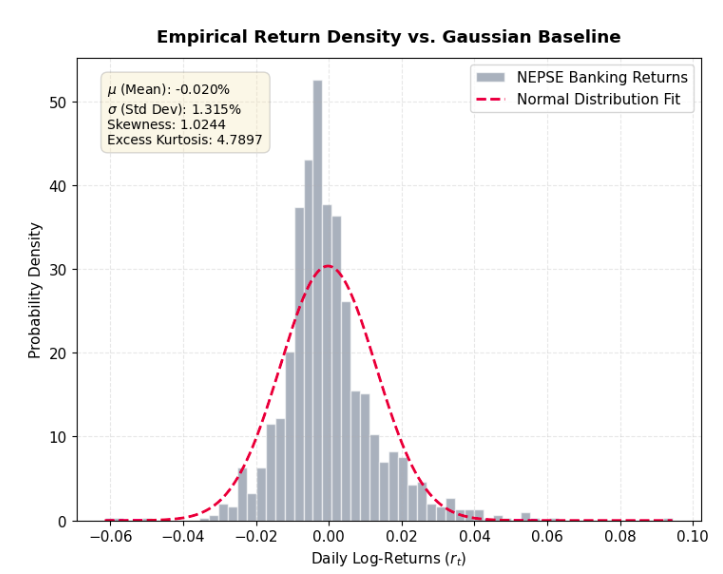
\includegraphics[width=0.8\textwidth]{figures/emperical-vs-gaussian.png}
\caption{Empirical return density vs. Gaussian baseline (leptokurtic peak).}
\label{fig:density}
\end{figure}

Figure \ref{fig:qq} (normal Q-Q plot) further highlights tail deviations: the sample quantiles depart from the 45° reference line, with extreme positive and negative returns lying far outside the Gaussian confidence bands. These empirical facts motivate the use of jump‑diffusion model.

\begin{figure}[H]
\centering
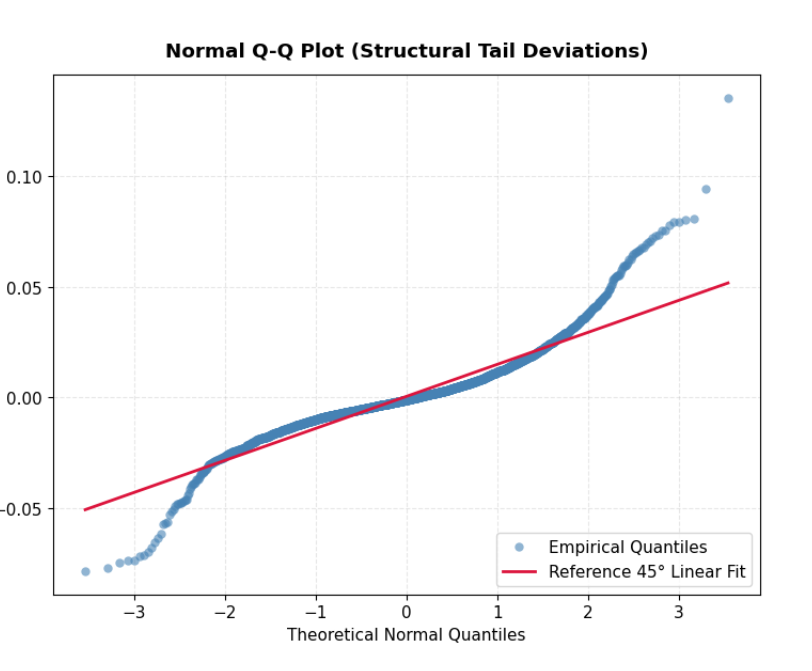
\includegraphics[width=0.8\textwidth]{figures/normal-q-q.png}
\caption{Normal Q-Q plot showing tail deviations.}
\label{fig:qq}
\end{figure}

\begin{table}[H]
\centering
\caption{Descriptive statistics and normality tests for NEPSE Commercial Banks daily log‑returns (October 2013 – June 2026).}
\label{tab:desc}
\begin{tabular}{l r}
\toprule
Statistic & Value \\
\midrule
Mean (daily) & $0.000424$ ($0.0424\%$) \\
Variance (daily) & $0.000235$ \\
Std. deviation (daily) & $0.015321$ ($1.5321\%$) \\
Skewness & $0.9029$ \\
Excess kurtosis & $7.2073$ \\
Jarque–Bera test & Stat $= 7981.75$, $p = 0.0000$ \\
Shapiro–Wilk test & Stat $= 0.8919$, $p = 0.0000$ \\
\bottomrule
\end{tabular}
\end{table}

\section{Time Series Dependence and ARCH Effects}
\paragraph{Serial correlation.}
The Ljung–Box test on raw returns (Table \ref{tab:serial}) shows significant autocorrelation at lags 10 and 20 ($p<0.001$), indicating that the mean equation requires an autoregressive structure. Squared returns exhibit even stronger dependence, with test statistics that are orders of magnitude larger and $p$-values virtually zero – clear evidence of volatility clustering.

\paragraph{ARCH effects.}
Engle’s ARCH Lagrange Multiplier test (lag 10) gives a statistic of $778.07$ ($p=1.07\times10^{-160}$), strongly rejecting the null of no conditional heteroskedasticity. This establishes a firm baseline for GARCH‑type variance dynamics.

Figure \ref{fig:acfpacf} displays the autocorrelation (ACF) and partial autocorrelation (PACF) of raw returns (top row) and squared returns (bottom row). For raw returns, only a few lags exceed the significance bands, suggesting weak but non‑negligible serial correlation. In contrast, the ACF of squared returns decays very slowly, remaining positive for more than 30 lags – a classic signature of long‑memory volatility clustering. The PACF of squared returns cuts off after a few lags, supporting an ARCH/GARCH specification.

\begin{figure}[H]
\centering
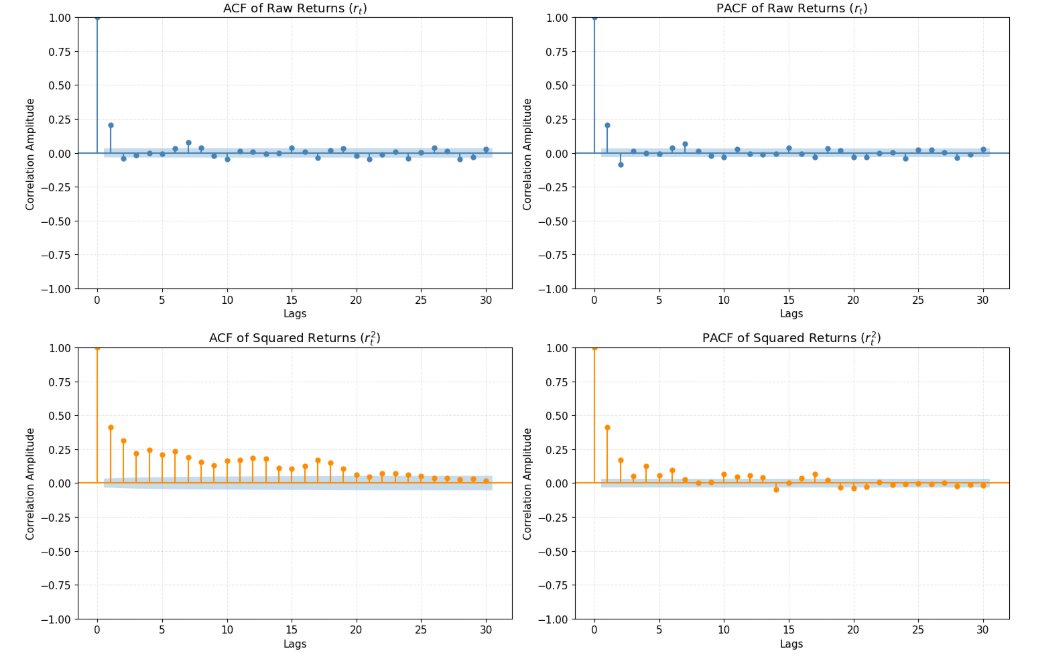
\includegraphics[width=0.8\textwidth]{figures/acf-pacf.png}
\caption{ACF and PACF of raw returns (mean equation) and squared returns (variance equation).}
\label{fig:acfpacf}
\end{figure}

Figure \ref{fig:volcluster} shows the raw log-returns with a rolling 21-day volatility corridor, visually confirming the alternating calm and turbulent periods characteristic of volatility clustering.

\begin{figure}[H]
\centering
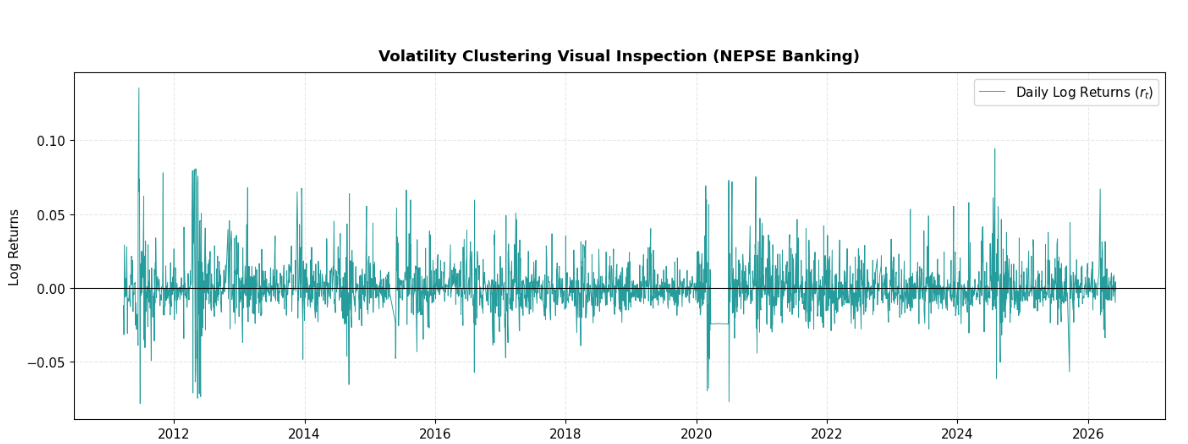
\includegraphics[width=0.8\textwidth]{figures/volatility-clustering-visual-inspection.png}
\caption{Volatility clustering visual inspection (log returns with 21‑day rolling volatility corridor).}
\label{fig:volcluster}
\end{figure}

\begin{table}[H]
\centering
\caption{Ljung–Box and ARCH tests for raw and squared returns (post‑break sample).}
\label{tab:serial}
\begin{tabular}{l c c}
\toprule
Test & Statistic & $p$-value \\
\midrule
LB (raw returns, lag 10) & $190.69$ & $0.0000$ \\
LB (raw returns, lag 20) & $208.99$ & $0.0000$ \\
LB (squared returns, lag 10) & $2015.56$ & $0.0000$ \\
LB (squared returns, lag 20) & $2720.19$ & $0.0000$ \\
Engle ARCH LM (lag 10) & $778.07$ & $0.0000$ \\
\bottomrule
\end{tabular}
\end{table}

\paragraph{Leverage effect.}
We examined the cross‑correlation between past returns $r_{t-k}$ and current absolute returns $|r_t|$ for $k=1,\dots,20$ days. The minimum correlation is $0.0088$ at lag 9, which lies inside the 95\% asymptotic confidence band $\pm 0.0333$. Hence no statistically significant leverage effect is present; negative and positive shocks have symmetric impacts on future volatility. A symmetric GARCH specification is therefore admissible.

\section{Stationarity and Ergodicity}
The Augmented Dickey–Fuller (ADF) test yields a statistic of $-11.4461$ ($p=6.01\times10^{-21}$), rejecting the unit‑root null. The KPSS test gives a statistic of $0.2225$ ($p>0.1$), failing to reject stationarity. Together, these results confirm that the log‑return series is strictly stationary and mean‑reverting, providing a solid foundation for time series modelling.

\section{Jump Detection and Structural Break}
\label{sec:break}
\paragraph{Jump identification.}
We apply a dynamic $3\sigma$ filter using a rolling 21‑day window to isolate outlier shocks. Figure \ref{fig:jumps} illustrates the detected jumps (red dots) against the daily log‑returns (grey line) and the rolling $3\sigma$ corridor (orange dashed). The plot shows that most large positive or negative returns are flagged as jumps, and these jumps are often followed by periods of elevated volatility. A total of $39$ jump events are detected, corresponding to $1.12\%$ of trading days. The annualised jump intensity (based on 252 trading days) is $\lambda_{\text{annual}} = 2.83$ jumps per year. The mean inter‑arrival time between jumps is $88.4$ trading days (median $75.5$ days), indicating that jumps occur roughly every four months.

\begin{figure}[H]
\centering
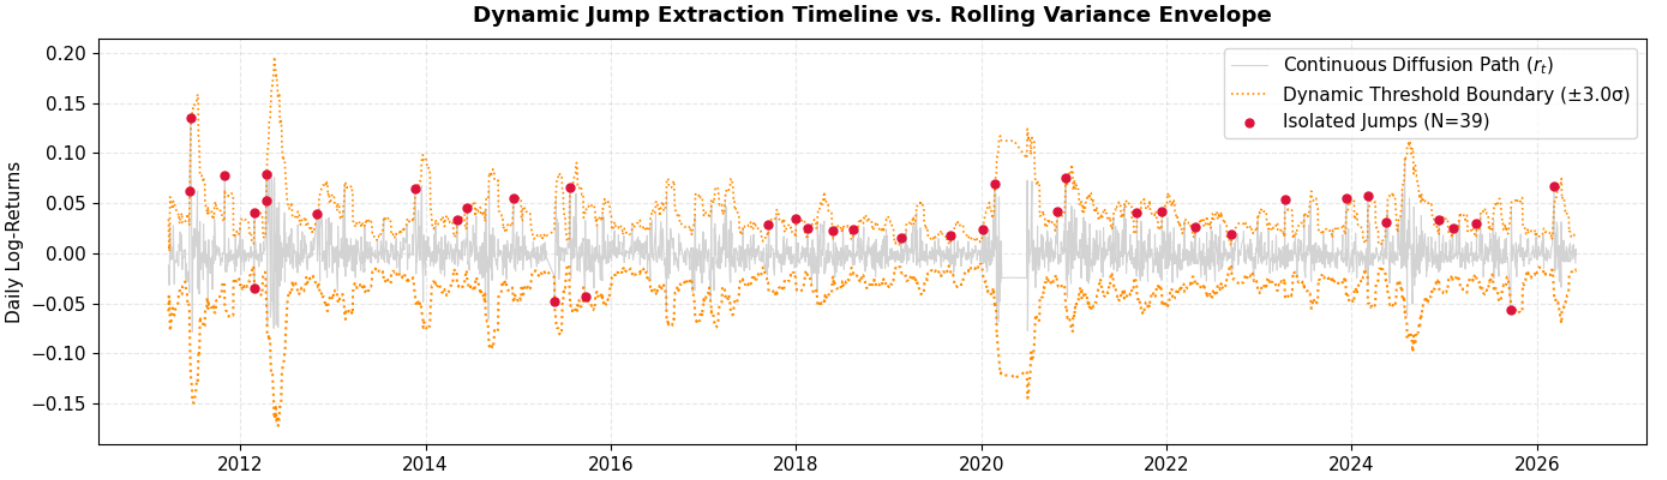
\includegraphics[width=0.8\textwidth]{figures/dynamic-jump.png}
\caption{Dynamic jump extraction timeline (rolling $3\sigma$ corridor and detected jumps).}
\label{fig:jumps}
\end{figure}

\paragraph{Structural break analysis.}
The Zivot–Andrews test on log prices (with one endogenous break) produces a test statistic of $-3.1718$ ($p=0.852$), failing to reject the unit‑root null. The estimated break date is \textbf{30 September 2013}. Figure \ref{fig:break} shows the log‑price series with a vertical line at the break point. While the test does not find a permanent regime shift, the break point is used to define a homogeneous sample for COGARCH estimation, as the pre‑break period (2012–2013) exhibits different dynamics. All subsequent analyses are therefore conducted on the post‑break sample (1 October 2013 – 3 June 2026).

\begin{figure}[H]
\centering
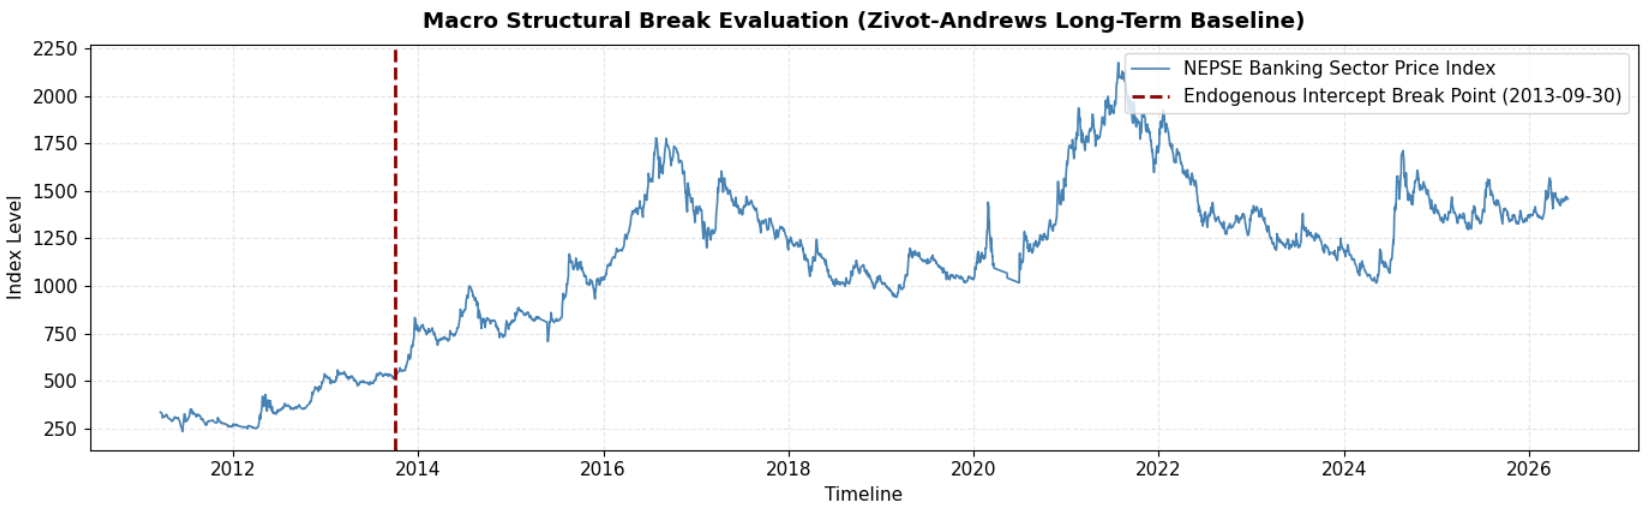
\includegraphics[width=0.8\textwidth]{figures/breakdown.png}
\caption{Macro Structural Break Evaluation (Zivot-Andrews Long-Term Baseline).}
\label{fig:break}
\end{figure}

\section{Empirical Chaos Diagnostics (Post‑Break Sample)}
\paragraph{Tail index.}
The Hill estimator applied to the top $5\%$ of absolute returns $|r_t|$ gives $\hat{\gamma}_{\text{ret}} = 2.7805 \pm 0.4542$. Figure \ref{fig:hill} displays the Hill tail index as a function of the number of order statistics $k$; the estimate stabilises around $k \approx 140$ (5\% of the sample), indicating robustness. This value characterises the power‑law decay of the return distribution; values above 2 suggest finite variance.

\begin{figure}[H]
\centering
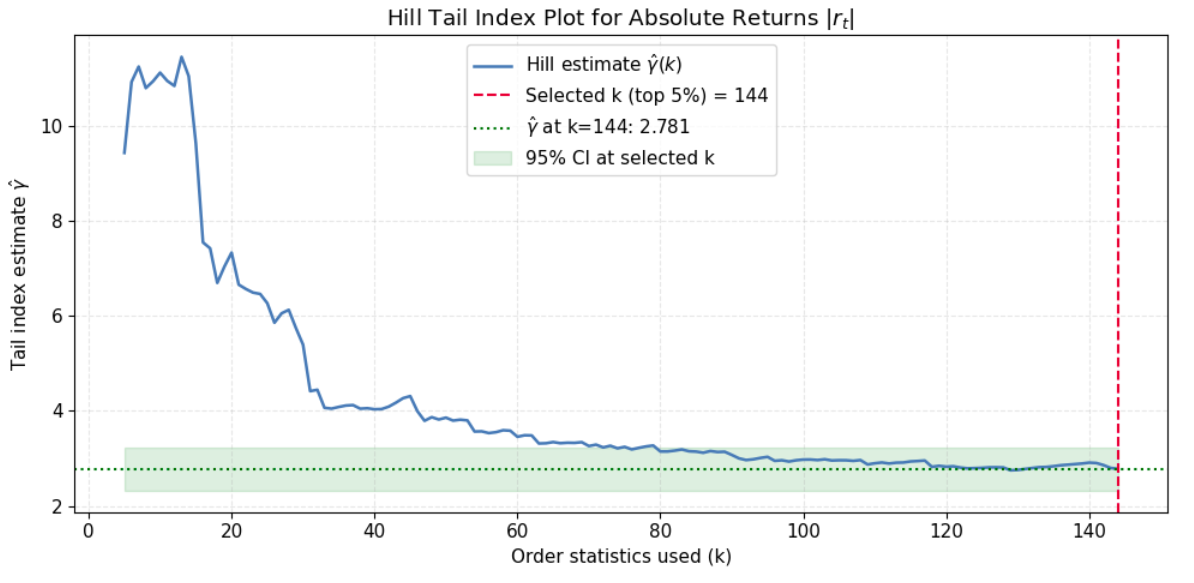
\includegraphics[width=0.8\textwidth]{figures/hill-tail-index.png}
\caption{Hill tail index plot for absolute returns $|r_t|$ (stability over $k$).}
\label{fig:hill}
\end{figure}

\paragraph{Long memory.}
Detrended fluctuation analysis (DFA) on $|r_t|$ yields a Hurst exponent $\hat{H} = 0.7751$, which exceeds $0.5$, confirming persistent long‑memory dynamics in absolute returns – a signature of volatility clustering that decays hyperbolically. Figure \ref{fig:hurst} shows the generalised Hurst exponent $H(q)$ from MF‑DFA: $H(q)$ decreases with $q$, confirming multifractality (discussed next).

\begin{figure}[H]
\centering
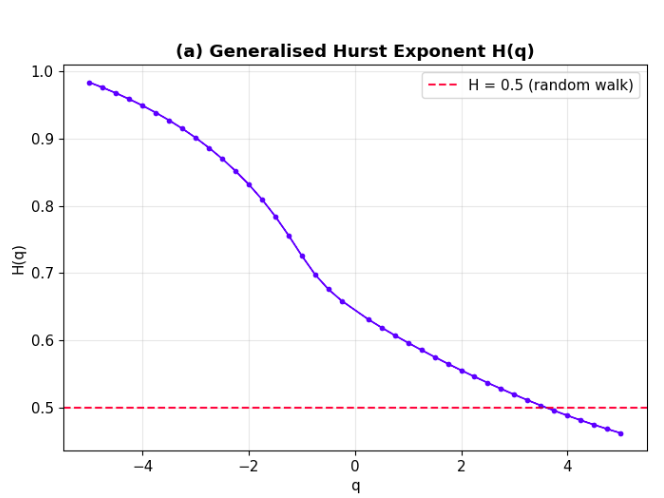
\includegraphics[width=0.8\textwidth]{figures/hurst-exponent.png}
\caption{Generalised Hurst Exponent $H(q)$ from MF‑DFA.}
\label{fig:hurst}
\end{figure}

\paragraph{Multifractality.}
Multifractal DFA (MF‑DFA) with $q\in[-5,5]$ reveals a decreasing generalised Hurst exponent $H(q)$ and a concave scaling function $\zeta(q)=qH(q)-1$, deviating from the linear monofractal benchmark. Figure \ref{fig:mf} presents the multifractal spectrum $f(\alpha)$ versus the Hölder exponent $\alpha$. The width of the spectrum is $\Delta\alpha = 0.7959$, indicating a rich cascade structure and multiple scaling regimes.

\begin{figure}[H]
\centering
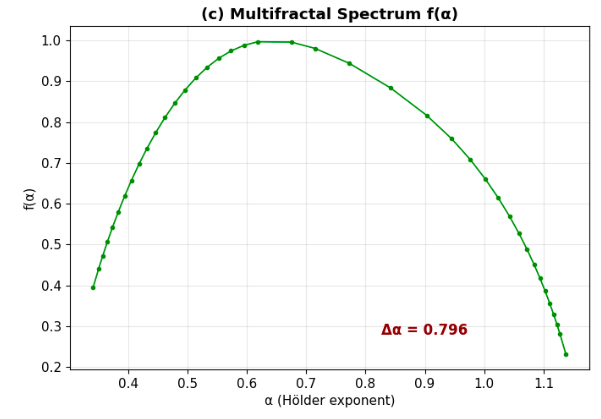
\includegraphics[width=0.8\textwidth]{figures/multi-fractal.png}
\caption{Multifractal spectrum $\alpha$ vs. $f(\alpha)$ from MF‑DFA.}
\label{fig:mf}
\end{figure}

These pre‑estimation diagnostics already point to nonlinear, non‑normal dynamics consistent with the COGARCH framework.
